%%*****************************************************************************
%% Copyright (c) 2008 Gerd Neugebauer
%%
%% Permission is granted to copy, distribute and/or modify this document
%% under the terms of the GNU Free Documentation License, Version 1.2
%% or any later version published by the Free Software Foundation;
%% with no Invariant Sections, no Front-Cover Texts, and no Back-Cover Texts.
%%
%%*****************************************************************************
%% $Id:bst-language.tex 7067 2008-05-18 11:06:56Z gene $
%%*****************************************************************************
%% Author: Gerd Neugebauer
%%-----------------------------------------------------------------------------

\chapter{The BST Language}%
\index{BST language|(}

\IM{08x1}%
The processing of the data base entries can be programmed with a small
special purpose programming language. Since it seems to have no name
it is called the BST language

Usually the instructions are read from a file. The default extension
of these files is \texttt{.bst}. The content is interpreted to produce
the formatted output.

The primary goal of \BibTeX\index{BibTeX@\BibTeX} is the processing of
bibliographic databases. Thus the language is tailored towards the
formatting of bibliographies.


\def\cmdIndex#1{\index{#1@\texttt{#1}}}%
\def\fctIndex#1{\index{#1@\texttt{#1}}%
  \index{function!#1@\texttt{#1}}}%
\def\varIndex#1{\index{#1@\texttt{#1}}%
  \index{variable!#1@\texttt{#1}}}%

\section{The Programming Model}

The BST language is based on a simple stack based metaphor. The stack
is the central data structure in the program. The stack is able to
carry arbitrary data. Especially it is possible to push code segments
to the stack.

\begin{figure}[tb]
  \centering
  %%*****************************************************************************
%% Copyright (c) 2008 Gerd Neugebauer
%%
%% Permission is granted to copy, distribute and/or modify this document
%% under the terms of the GNU Free Documentation License, Version 1.2
%% or any later version published by the Free Software Foundation;
%% with no Invariant Sections, no Front-Cover Texts, and no Back-Cover Texts.
%%
%%*****************************************************************************
%% $Id:bst-model.tex 7067 2008-05-18 11:06:56Z gene $
%%*****************************************************************************
%% Author: Gerd Neugebauer
%%-----------------------------------------------------------------------------
\begingroup
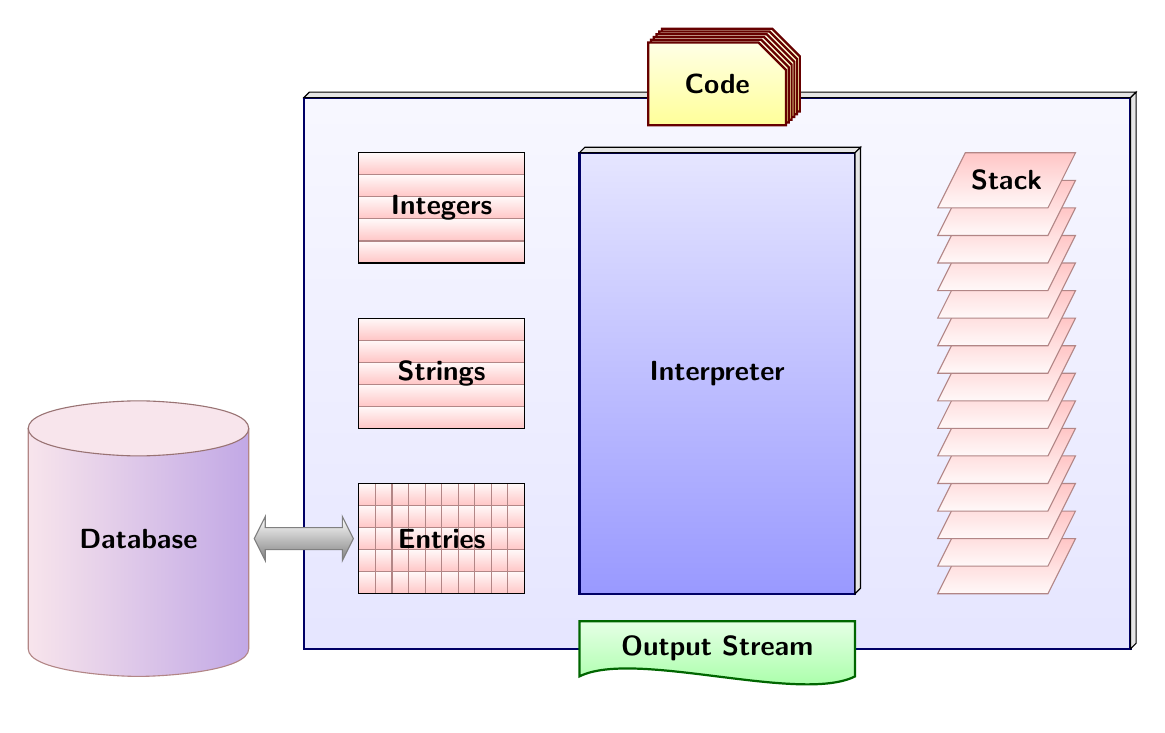
\begin{tikzpicture}[scale=.7]\sf\bfseries
  % --- bottom layer ---
  \shade[top color=white!97!blue,bottom color=white!90!blue,draw=blue!40!black,thick]
  (0,0) rectangle (15,10);
  \draw[fill=gray!20!white] (0,10) -- (.1,10.1) -- (15.1,10.1) -- (15,10) -- cycle;
  \draw[fill=gray!20!white] (15,10) -- (15.1,10.1) -- (15.1,.1) -- (15,0) -- cycle;

  % --- code ---
  \begin{scope}[shift={(6.25,9.5)},scale=.5]
    \begin{scope}[shift={(.5,.5)}]
      \shade[top color=white!90!yellow,bottom color=white!60!yellow,draw=red!40!black,thick]
      (0,0) -- (5,0) -- (5,2) -- (4,3) -- (0,3) -- cycle;
    \end{scope}
    \begin{scope}[shift={(.4,.4)}]
      \shade[top color=white!90!yellow,bottom color=white!60!yellow,draw=red!40!black,thick]
      (0,0) -- (5,0) -- (5,2) -- (4,3) -- (0,3) -- cycle;
    \end{scope}
    \begin{scope}[shift={(.3,.3)}]
      \shade[top color=white!90!yellow,bottom color=white!60!yellow,draw=red!40!black,thick]
      (0,0) -- (5,0) -- (5,2) -- (4,3) -- (0,3) -- cycle;
    \end{scope}
    \begin{scope}[shift={(.2,.2)}]
      \shade[top color=white!90!yellow,bottom color=white!60!yellow,draw=red!40!black,thick]
      (0,0) -- (5,0) -- (5,2) -- (4,3) -- (0,3) -- cycle;
    \end{scope}
    \begin{scope}[shift={(.1,.1)}]
      \shade[top color=white!90!yellow,bottom color=white!60!yellow,draw=red!40!black,thick]
      (0,0) -- (5,0) -- (5,2) -- (4,3) -- (0,3) -- cycle;
    \end{scope}
    \shade[top color=white!90!yellow,bottom color=white!60!yellow,draw=red!40!black,thick]
    (0,0) -- (5,0) -- (5,2) -- (4,3) -- (0,3) -- cycle;
  \end{scope}
  \draw (7.5,10.25) node {Code};

  % --- interpreter ---
  \shade[top color=white!90!blue,bottom color=white!60!blue,draw=blue!40!black,thick]
  (5,1) rectangle (10,9);
  \draw[fill=gray!20!white] (5,9) -- (5.1,9.1) -- (10.1,9.1) -- (10,9) -- cycle;
  \draw[fill=gray!20!white] (10,9) -- (10.1,9.1) -- (10.1,1.1) -- (10,1) -- cycle;
  \draw (7.5,5) node {Interpreter};
  
  \shade[top color=white!90!green,bottom color=white!60!green,draw=green!40!black,thick]
  (5,-.5) .. controls (6,0) and (9,-1) .. (10,-.5) -- (10,.5) -- (5,.5) -- cycle;
  \draw (7.5,0) node {Output Stream};


  % --- stack ---
  \shade[top color=white!10!pink,bottom color=white!90!pink,draw=pink!70!black,shift={(11.5,1)}] (0,0) -- (.5,1) -- (2.5,1) -- (2,0) -- cycle;
  \shade[top color=white!10!pink,bottom color=white!90!pink,draw=pink!70!black,shift={(11.5,1.5)}] (0,0) -- (.5,1) -- (2.5,1) -- (2,0) -- cycle;
  \shade[top color=white!10!pink,bottom color=white!90!pink,draw=pink!70!black,shift={(11.5,2)}] (0,0) -- (.5,1) -- (2.5,1) -- (2,0) -- cycle;
  \shade[top color=white!10!pink,bottom color=white!90!pink,draw=pink!70!black,shift={(11.5,2.5)}] (0,0) -- (.5,1) -- (2.5,1) -- (2,0) -- cycle;
  \shade[top color=white!10!pink,bottom color=white!90!pink,draw=pink!70!black,shift={(11.5,3)}] (0,0) -- (.5,1) -- (2.5,1) -- (2,0) -- cycle;
  \shade[top color=white!10!pink,bottom color=white!90!pink,draw=pink!70!black,shift={(11.5,3.5)}] (0,0) -- (.5,1) -- (2.5,1) -- (2,0) -- cycle;
  \shade[top color=white!10!pink,bottom color=white!90!pink,draw=pink!70!black,shift={(11.5,4)}] (0,0) -- (.5,1) -- (2.5,1) -- (2,0) -- cycle;
  \shade[top color=white!10!pink,bottom color=white!90!pink,draw=pink!70!black,shift={(11.5,4.5)}] (0,0) -- (.5,1) -- (2.5,1) -- (2,0) -- cycle;
  \shade[top color=white!10!pink,bottom color=white!90!pink,draw=pink!70!black,shift={(11.5,5)}] (0,0) -- (.5,1) -- (2.5,1) -- (2,0) -- cycle;
  \shade[top color=white!10!pink,bottom color=white!90!pink,draw=pink!70!black,shift={(11.5,5.5)}] (0,0) -- (.5,1) -- (2.5,1) -- (2,0) -- cycle;
  \shade[top color=white!10!pink,bottom color=white!90!pink,draw=pink!70!black,shift={(11.5,6)}] (0,0) -- (.5,1) -- (2.5,1) -- (2,0) -- cycle;
  \shade[top color=white!10!pink,bottom color=white!90!pink,draw=pink!70!black,shift={(11.5,6.5)}] (0,0) -- (.5,1) -- (2.5,1) -- (2,0) -- cycle;
  \shade[top color=white!10!pink,bottom color=white!90!pink,draw=pink!70!black,shift={(11.5,7)}] (0,0) -- (.5,1) -- (2.5,1) -- (2,0) -- cycle;
  \shade[top color=white!10!pink,bottom color=white!90!pink,draw=pink!70!black,shift={(11.5,7.5)}] (0,0) -- (.5,1) -- (2.5,1) -- (2,0) -- cycle;
  \shade[top color=white!10!pink,bottom color=white!90!pink,draw=pink!70!black,shift={(11.5,8)}] (0,0) -- (.5,1) -- (2.5,1) -- (2,0) -- cycle;
  \draw (12.75,8.5) node {Stack};

  % --- integers ---
  \shade[top color=white!90!pink,bottom color=white!10!pink,draw=pink!70!black]
  (1,7) rectangle (4,7.4);
  \shade[shift={(0,.4)},top color=white!90!pink,bottom color=white!10!pink,draw=pink!70!black]
  (1,7) rectangle (4,7.4);
  \shade[shift={(0,.8)},top color=white!90!pink,bottom color=white!10!pink,draw=pink!70!black]
  (1,7) rectangle (4,7.4);
  \shade[shift={(0,1.2)},top color=white!90!pink,bottom color=white!10!pink,draw=pink!70!black]
  (1,7) rectangle (4,7.4);
  \shade[shift={(0,1.6)},top color=white!90!pink,bottom color=white!10!pink,draw=pink!70!black]
  (1,7) rectangle (4,7.4);
  \draw (1,7) rectangle (4,9);
  \draw (2.5,8) node {Integers};

  % --- strings ---
  \shade[top color=white!90!pink,bottom color=white!10!pink,draw=pink!70!black]
  (1,4) rectangle (4,4.4);
  \shade[shift={(0,.4)},top color=white!90!pink,bottom color=white!10!pink,draw=pink!70!black]
  (1,4) rectangle (4,4.4);
  \shade[shift={(0,.8)},top color=white!90!pink,bottom color=white!10!pink,draw=pink!70!black]
  (1,4) rectangle (4,4.4);
  \shade[shift={(0,1.2)},top color=white!90!pink,bottom color=white!10!pink,draw=pink!70!black]
  (1,4) rectangle (4,4.4);
  \shade[shift={(0,1.6)},top color=white!90!pink,bottom color=white!10!pink,draw=pink!70!black]
  (1,4) rectangle (4,4.4);
  \draw (1,4) rectangle (4,6);
  \draw (2.5,5) node {Strings};

  % --- entries ---
  \shade[top color=white!90!pink,bottom color=white!10!pink,draw=pink!70!black]
  (1,1) rectangle (4,1.4);
  \shade[shift={(0,.4)},top color=white!90!pink,bottom color=white!10!pink,draw=pink!70!black]
  (1,1) rectangle (4,1.4);
  \shade[shift={(0,.8)},top color=white!90!pink,bottom color=white!10!pink,draw=pink!70!black]
  (1,1) rectangle (4,1.4);
  \shade[shift={(0,1.2)},top color=white!90!pink,bottom color=white!10!pink,draw=pink!70!black]
  (1,1) rectangle (4,1.4);
  \shade[shift={(0,1.6)},top color=white!90!pink,bottom color=white!10!pink,draw=pink!70!black]
  (1,1) rectangle (4,1.4);
  \draw[shift={(.3,0)},draw=pink!70!black] (1,1) -- (1,3);
  \draw[shift={(.6,0)},draw=pink!70!black] (1,1) -- (1,3);
  \draw[shift={(.9,0)},draw=pink!70!black] (1,1) -- (1,3);
  \draw[shift={(1.2,0)},draw=pink!70!black] (1,1) -- (1,3);
  \draw[shift={(1.5,0)},draw=pink!70!black] (1,1) -- (1,3);
  \draw[shift={(1.8,0)},draw=pink!70!black] (1,1) -- (1,3);
  \draw[shift={(2.1,0)},draw=pink!70!black] (1,1) -- (1,3);
  \draw[shift={(2.4,0)},draw=pink!70!black] (1,1) -- (1,3);
  \draw[shift={(2.7,0)},draw=pink!70!black] (1,1) -- (1,3);
  \draw (1,1) rectangle (4,3);
  \draw (2.5,2) node {Entries};

  \begin{scope}[shift={(-5,0)}]
    \shade[left color=white!96!blue!70!pink,right color=white!60!blue!60!pink,draw=pink!70!black]
    (0,0)   .. controls (0,-.4) and (1.5,-.5) ..
    (2,-.5)  .. controls (2.5,-.5) and (4,-.4) ..
    (4,0) -- (4,4) -- (0,4) -- cycle;
    \draw[shift={(0,4)},fill=white!96!blue!70!pink,draw=pink!60!black]
    (0,0)   .. controls (0,.4) and (1.5,.5) ..
    (2,.5)  .. controls (2.5,.5) and (4,.4) ..
    (4,0)   .. controls (4,-.4) and (2.5,-.5) ..
    (2,-.5) .. controls (1.5,-.5) and (0,-.4) ..
    (0,0);
  \end{scope}
  \draw (-3,2) node {Database};

%  \draw[shift={(0,-5)}]
%  (-.2,0) -- (0,.4) -- (0,.2) -- (1,.2) -- (1,.4) -- (1.2,0) --
%  (1,-.4) -- (1,-.2) -- (0,-.2) -- (0,-.4) -- cycle;

  \shade[shift={(-.7,2)}, top color=white, bottom color=gray,draw=gray]
  (-.2,0) -- (0,.4) -- (0,.2) -- (1.4,.2) -- (1.4,.4) -- (1.6,0) --
  (1.4,-.4) -- (1.4,-.2) -- (0,-.2) -- (0,-.4) -- cycle;

\end{tikzpicture}
\endgroup
\endinput
%
% Local Variables: 
% mode: latex
% TeX-master: nil
% End: 

  \caption{The BST Programming Model}
  \label{fig:bst-model}
\end{figure}


\subsection{The Database Context}

Whenever a bst program is executed a database is at hand. The program
has access to this database. The database contains a list of entries.
Those entries are filtered according to the citations given.


\subsection{Entries}

Entries tie together the information for one key. It has a set of
fields. Some of the fields are visible in the BST program. The fields
visible are defined with the command \texttt{entry} (see
section~\ref{sec:entry}).


\subsubsection{The Variable \texttt{sort.key\$}}%
\varIndex{sort.key\$}

One entry local variable predefined is the string-valued variable
\texttt{sort.key\$}. It is used to sort the entries with the command
\texttt{sort} (see section~\ref{sec:sort}).


\subsubsection{The Variable \texttt{locator.resource\$}}%
\varIndex{locator.resource\$}

\IM{x}%
Each entry carries the information where it has been defined. The
string-valued variable \texttt{locator.resource\$}. it contains the
name of the resource this entry is coming from. The string contained
is the name as given in the \Macro{bibdata} declaration in the aux
file. This means it doe not reflect the actual resource resolution as
performed by the resource loading. Thus this variable is not
implementation dependant.


\subsubsection{The Variable \texttt{locator.line\$}}%
\varIndex{locator.line\$}

\IM{x}%
Each entry carries the information where it has been defined. The
string-valued variable \texttt{locator.line\$}. it contains the line
number in the resource from which this entry is coming from.


\subsection{Global Integers}

The processor for the BST language has a global storage for variables.
First of all there are integer valued variables. The command
\texttt{integers} (see section~\ref{sec:integers}) can be used to
define integer variables.


\subsubsection{The Variable \texttt{entry.max\$}}%
\varIndex{entry.max\$}

The global integer variable \texttt{entry.max\$} is predefined. It
contains the maximal number of entries. It is fed from a
configuration.

In \ExBib\index{ExBib@\ExBib} it contains a large number which does
not have any influence on the number of entries. It is defined for
backward compatibility only.

\subsubsection{The Variable \texttt{global.max\$}}%
\varIndex{global.max\$}

The global integer variable \texttt{global.max\$} is predefined. It
contains the maximal length of strings. It is fed from a
configuration.

In \ExBib\index{ExBib@\ExBib} it contains a large number which does
not have any influence on the length of strings. It is defined for
backward compatibility only.


\subsection{Global Strings}

The processor for the BST language has a global storage for variables.
Beside the integer valued variables there are string valued variables.
The command \texttt{strings} (see section~\ref{sec:bst.strings}) can be
used to define global string variables.

There are no global string variables predefined.


\section{Syntax}

The bst source code follows some very simple syntax rules. There are
only a few characters beside white-space which have a special meaning:

\begin{itemize}
\item The percent sign \verb|%| starts an endline comment (see
  section~\ref{sec:bst.comments}).
\item The double quote sign \verb|"| starts a string literal (see
  section~\ref{sec:bst.strings}).
\item The hash amrk \verb|#| starts an integer literal (see
  section~\ref{sec:bst.integers}).
\item The single quote sign \verb|'| quotes a following literal (see
  section~\ref{sec:bst.quote}).
\item The braces \verb|{| and \verb|}| enclose arguments and code (see
  section~\ref{sec:bst.code}).
\end{itemize}


\subsection{Comments}\label{sec:bst.comments}

Comments in a bst file are started with a percent sign (\verb|%|) and
continues to the end of the line. This is the same definition an in
\TeX\index{TeX@\TeX}.

The following example is taken from \File{alpha.bst}:

\begin{lstlisting}[language=bst]
  % BibTeX standard bibliography style `alpha'
\end{lstlisting}


\subsection{String Literals}\label{sec:bst.strings}

String literals in the code are enclose in double quotes '"'. The
strings contain braces only in matching pairs. As a consequence a
double quote can be included in a string by enclosing it in braces.
This is shown in the following example:

\begin{lstlisting}[language=bst,escapechar=|]
  "abc {|\char`\"|} def"
\end{lstlisting}


\subsection{Integer Literals}\label{sec:bst.integers}

Integer literals in the code are preceded by a hash mark '\#'.

\begin{lstlisting}[language=bst]
  #123
\end{lstlisting}

Integers can be negative. In this case the sign is written after the
initial hash mark:

\begin{lstlisting}[language=bst]
  #-123
\end{lstlisting}


\subsection{Quoting}\label{sec:bst.quote}

Ususally any symbol appearing in the program is replaced by its value
upon evaluation. There are situations where an expansion is not
desirable. For instance to set a variable to a value you have to
specify the variable itself and not its value. For this purpose
symbols can be quoted. This is done by preceding the symbol by a
aingle quote \verb|'|.

\begin{lstlisting}[language=bst]
  'abc
\end{lstlisting}

In this case the symbol is pushed to the stack instead of its value.

\subsection{Code}\label{sec:bst.code}

Code dnoted a list of function invocations. Code is enclosed in
braces. When code is encountered during the evaluation of a program it
is simply pushed onto the stack.

\begin{lstlisting}[language=bst]
  { skip$ }
\end{lstlisting}

\section{Expansion of Variables and Fields}

Local variables and entry variables -- both integer valued or string
valued -- as well as fields are replaced by their value before this
value is pushed to the stack.

All these entities share the same name space. This means that there
can not be two different variables with the same name.


\section{Commands}

\subsection{The \texttt{entry} Declaration}%
\cmdIndex{entry}%
\label{sec:entry}

The declaration defines the view to an entry. For this purpose it
defines which fields are defined. In addition it defines the list of
integer entry variables and string entry variables. Thus the entry
declaration has three arguments in braces. The first one is the list
of fields the second one the list of integer entry variables and the
third the list of string entry variables. The elements of the lists
are separated by whitespace.

The fields, the entry variables and the global variables share a
common name space. Thus any name has to be unique among those.

The following example is taken from \File{alpha.bst}:

\begin{lstlisting}[language=bst]
  ENTRY
  { address
    author
    booktitle
    chapter
    edition
    editor
    howpublished
    institution
    journal
    key
    month
    note
    number
    organization
    pages
    publisher
    school
    series
    title
    type
    volume
    year
  }
  {}
  { label extra.label sort.label }
\end{lstlisting}


\subsection{The \texttt{integers} Declaration}%
\cmdIndex{integers}%
\label{sec:integers}

This declaration defines a set of global integers. It has one
argument. The argument contains a list of variable names separated by
white-space. The names must not collide with entry local strings,
entry local integers, global strings, and fields.

There may be any number of declarations of integer variables.
Nevertheless the declaration of a variable should precede its use.

The following example is taken from \File{alpha.bst}:

\begin{lstlisting}[language=bst]
  INTEGERS { output.state before.all }
\end{lstlisting}


\subsection{The \texttt{strings} Declaration}
\cmdIndex{strings}

This declaration defines a set of global strings. It has one argument.
The argument contains a list of variable names separated by
white-space. The names miust not collide with entry local strings,
entry local integers, global integers, and fields.

There may be any number of declarations of string variables.
Nevertheless the declaration of a variable should precede its use.

The following example is taken from \File{alpha.bst}:

\begin{lstlisting}[language=bst]
  STRINGS { s t }
\end{lstlisting}


\subsection{The \texttt{macro} Declaration}
\cmdIndex{macro}

This declaration defines a macro. It takes two arguments -- the name
of the macro and its value. The value is an expression which evaluates
to a string.

This declaration has the same effect as the definition of a macro with
the \texttt{@string} declaration in a bib file.

The following example is taken from \File{alpha.bst}:

\begin{lstlisting}[language=bst]
  MACRO {jan} {"January"}
\end{lstlisting}


\subsection{The \texttt{execute} Command}
\cmdIndex{execute}

This command executes the function in the argument. There is no
current entry then this code is executed.

The following example is taken from \File{alpha.bst}:

\begin{lstlisting}[language=bst]
  EXECUTE {begin.bib}
\end{lstlisting}


\subsection{The \texttt{iterate} Command}
\cmdIndex{iterate}

This command iterates over the entries in the order they are currently
in the entry list from the beginning to the end. Each entry is
considered as current entry and the function in the argument is
executed.

The following example is taken from \File{alpha.bst}:

\begin{lstlisting}[language=bst]
  ITERATE{call.type$}
\end{lstlisting}


\subsection{The \texttt{reverse} Command}
\cmdIndex{reverse}

This command iterates over the entries in the reverse order they are
currently in the entry list from the beginning to the end. Each entry
is considered as current entry and the function in the argument is
executed.

The following example is taken from \File{alpha.bst}:

\begin{lstlisting}[language=bst]
  REVERSE{reverse.pass}
\end{lstlisting}


\subsection{The \texttt{sort} Command}
\cmdIndex{sort}%
\label{sec:sort}

This command sorts the entries of the database according to its sort
key lexicographically increasing. The sort key is taken from the entry
variable \texttt{sort.key\$}.

\begin{lstlisting}[language=bst]
  SORT
\end{lstlisting}


\subsection{The \texttt{read} Command}
\cmdIndex{read}

This command read entries into the database. The database is empty
before the read command is encountered. The list of entries is ordered
according to the order they are encountered.

\begin{lstlisting}[language=bst]
  READ
\end{lstlisting}


\subsection{The \texttt{function} Definition}
\cmdIndex{function}

This declaration defines a user defined function. It takes two
arguments which are the name of the function and the code associated
with it.

\begin{lstlisting}[language=bst]
  FUNCTION {sortify}
  { purify$
    "l" change.case$
  }
\end{lstlisting}\fctIndex{purify\$}\fctIndex{change.case\$}


\subsection{The \texttt{input} Command}
\cmdIndex{input}

The command takes one argument containg the name of another bst file.
This bst file is read in in place of this instruction as if the
contents of those file would have been included here. \IM{x}

If the named file or other resource could not be found then an error
is raised.

\begin{lstlisting}[language=bst]
  INPUT{some/other/bst}
\end{lstlisting}


\subsection{The \texttt{option} Declaration}
\cmdIndex{option}

The command takes three arguments. The first one is the type
indicator. It takes the values \texttt{integer} or \texttt{string}. In
the first case an integer-valued option is defined and in the second
case a string-valued option. The second argument is the name of the
option. it is enclosed on braces. Finally the third argument is the
value. It is also enclosed in braces. In the case of an integer it has
to be an integer constant as allowed in other placed of a BST file as
well. If the option is a string-valued option then all characters in
the balenced braces make up the value.\IM{x}

The following example shows both forms:

\begin{lstlisting}[language=bst]
  OPTION INTEGER{the-name}{#-123}
  OPTION STRING{the-other-name}{the value of the option}
\end{lstlisting}

The option declaration provides access from the BST program to the
options declared with \verb|\biboptions|. The value provided in the
declaration is a fallback which is used in case that the option is not
provided from outside.

In a function the value of an option can be pushed to the stack with
the name given to it. Thus the name must not be identical to the name
of a function or variable of some kind.


%------------------------------------------------------------------------------
\def\BstArg#1#2#3{
  \begin{scope}[shift={(#1,#2)}]
    \shade[top color=white!10!pink,bottom color=white!90!pink,draw=pink!70!black]
    (0,0) -- (.5,1.1) -- (4.5,1.1) -- (4,0) -- cycle;
    \draw (2.25,.55) node{#3};
  \end{scope}
}%
\def\BstStream(#1)#2{
  \begin{scope}[shift={(#1)}]
    \shade[top color=white!90!green,bottom color=white!60!green,draw=green!40!black,thick]
    (5,-.5) .. controls (6,0) and (9,-1) .. (10,-.5) -- (10,.5) -- (5,.5) -- cycle;
    \draw (7.5,0) node {#2};
  \end{scope}
}%
\newenvironment{BstFunction}[1]{\bigskip\par
  \def\In##1##2{\BstArg0{##1}{##2}}%
  \def\Out##1##2{\BstArg{11}{##1}{##2}}%
  \def\Stream##1{\BstStream(12,0.5){##1}}%
  \begin{tikzpicture}[scale=.5]\sf\itshape\scriptsize
    \draw[fill=white,dashed,draw = gray]
    (0,0) -- (.5,1.1) -- (4.5,1.1) -- (4,0) -- cycle;
    \draw[gray] (2.25,.55) node{ Stack};
    % ---
    \begin{scope}[shift={(5,0)},scale=.25]
      \begin{scope}[shift={(0.5,-0.5)}]
        \draw[thick,color=white!80!gray,fill==white!70!gray]
        (0.5,1) -- (19.5,1) -- (19,0) -- (21,2) -- (21.5,4) -- (20.5,3) --
        (1.5,3) -- cycle;
      \end{scope}
      \shade[top color=white!90!gray,bottom color=white!60!gray,draw=gray!40!black,thick]
      (0.5,1) -- (19.5,1) -- (19,0) -- (21,2) -- (21.5,4) -- (20.5,3) --
      (1.5,3) -- cycle;
      \draw (11.5,5) node{#1};
    \end{scope}
    % ---
    \begin{scope}[shift={(11,0)}]
      \draw[fill=white,dashed,draw = gray]
      (0,0) -- (.5,1.1) -- (4.5,1.1) -- (4,0) -- cycle;
      \draw[gray] (2.25,.55) node{ Stack};
    \end{scope}
  }{%
  \end{tikzpicture}%
  \bigskip\par
}%


\section{Functions}

The built-in functions are the basic building blocks for user defined
functions.

\subsection{The Function \texttt{>}}%
\fctIndex{>}

This function pops two numeric arguments from the stack and
compares them. It succeeds if the first argument is less than the
second argument. In case of success the integer 1 is pushed otherwise
the integer 0.

If the stack does not contain enough items or the arguments are not
integers then an error is raised.

\begin{BstFunction}{>}
  \In1{arg2}
  \In2{arg1}
  \Out1{boolean}
\end{BstFunction}

The following example is taken from \File{alpha.bst}:

\begin{lstlisting}[language=bst]
    { namesleft #0 > }
    { 
      % some actions

      namesleft #1 - 'namesleft :=
    }
  while$
\end{lstlisting}


\subsection{The Function \texttt{<}}%
\fctIndex{<}

This function pops two numeric arguments from the stack and
compares them. It succeeds if the first argument is greater than the
second argument. In case of success the integer 1 is pushed otherwise
the integer 0.

If the stack does not contain enough items or the arguments are not
integers then an error is raised.

\begin{BstFunction}{<}
  \In1{arg2}
  \In2{arg1}
  \Out1{boolean}
\end{BstFunction}

The following example is taken from \File{alpha.bst}:

\begin{lstlisting}[language=bst]
FUNCTION {tie.or.space.connect}
{ duplicate$ text.length$ #3 <
    { "~" }
    { " " }
  if$
  swap$ * *
}
\end{lstlisting}\fctIndex{<}\fctIndex{*}%
\fctIndex{duplicate\$}\fctIndex{if\$}\fctIndex{swap\$}\fctIndex{text.length\$}


\subsection{The Function \texttt{=}}%
\fctIndex{=}

This function pops two arguments from the stack and compares them.
If the arguments are integers then it succeeds if the first argument is
equal to the second argument. If the arguments are strings then it
succeeds if both strings contain the same characters. In case of
success the integer 1 is pushed otherwise the integer 0.

If the stack does not contain enough items or the arguments have
incomparable types then an error is raised.

\begin{BstFunction}{=}
  \In1{arg2}
  \In2{arg1}
  \Out1{boolean}
\end{BstFunction}

The following example is taken from \File{alpha.bst}:

\begin{lstlisting}[language=bst]
    output.state mid.sentence =
    { "number" }
    { "Number" }
  if$
\end{lstlisting}


\subsection{The Function \texttt{+}}%
\fctIndex{+}

This function pops two numeric arguments from the stack and
pushes back the sum of the two numbers to the stack.

If the stack does not contain enough items or the arguments are not
integers then an error is raised.

\begin{BstFunction}{+}
  \In1{arg2}
  \In2{arg1}
  \Out1{sum}
\end{BstFunction}

The following example is taken from \File{alpha.bst}:

\begin{lstlisting}[language=bst]
    s len #1 +
\end{lstlisting}


\subsection{The Function \texttt{-}}%
\fctIndex{-}

This function pops two numeric arguments from the stack and
pushes back the difference of the two numbers to the stack.

If the stack does not contain enough items or the arguments are not
integers then an error is raised.

\begin{BstFunction}{-}
  \In1{arg2}
  \In2{arg1}
  \Out1{difference}
\end{BstFunction}

The following example is taken from \File{alpha.bst}:

\begin{lstlisting}[language=bst]
  namesleft #1 - 'namesleft :=
\end{lstlisting}\fctIndex{-}\fctIndex{:=}


\subsection{The Function \texttt{*}}%
\fctIndex{*}

This function takes two string arguments from the stack and pushes the
concatenated string back to the stack. If not enough arguments are on
the stack or the arguments are no strings then an error is raised.

\begin{BstFunction}{*}
  \In1{arg2}
  \In2{arg1}
  \Out1{concatenated}
\end{BstFunction}

The following example is taken from \File{alpha.bst}:

\begin{lstlisting}[language=bst]
  "there's a month but no year in " cite$ * warning$
\end{lstlisting}


\subsection{The Function \texttt{:=}}%
\fctIndex{:=}

This function assigns a value to a variable or field. It takes two
arguments from the stack. The first argument is the name of the
target. In general it needs to be quoted (see
section~\ref{sec:bst.quote}). The second argument is the appropriate
value.

\begin{BstFunction}{:=}
  \In1{value}
  \In2{name}
\end{BstFunction}

The following example is taken from \File{alpha.bst}:

\begin{lstlisting}[language=bst]
    { namesleft #0 > }
    { 
      % some actions

      namesleft #1 - 'namesleft :=
    }
  while$
\end{lstlisting}\fctIndex{>}\fctIndex{-}\fctIndex{:=}\fctIndex{while\$}


\subsection{The Function \texttt{add.period\$}}%
\fctIndex{add.period\$}

This function pops a string argument from the stack and inspects it.
It the argument ends in one of the characters period '.', exclamation
mark '!', or question mark '?' then the argument is pushed back to the
stack. Otherwise a period '.' is added to the argument and the result
pushed to the stack.

When determining the last character closing braces are ignored.

\begin{BstFunction}{add.period\$}
  \In1{string}
  \Out1{result}
\end{BstFunction}

The following example is taken from \File{alpha.bst}:

\begin{lstlisting}[language=bst]
  FUNCTION {fin.entry}
  { add.period$
    write$
    newline$
  }
\end{lstlisting}\fctIndex{add.period\$}\fctIndex{write\$}\fctIndex{newline\$}


\subsection{The Function \texttt{call.type\$}}%
\fctIndex{call.type\$}

This function looks at the current entry and calls the function
with the same name as the type. The name is normalized; i.e.
translated to lower case.

If no such function is defined then the user-defined function
\fctIndex{default.type} is consulted and invoked instead.

\begin{BstFunction}{call.type\$}
\end{BstFunction}

The following example is taken from \File{alpha.bst}:

\begin{lstlisting}[language=bst]
  ITERATE {call.type$}
\end{lstlisting}


\subsection{The Function \texttt{change.case\$}}%
\fctIndex{change.case\$}

This function performs case conversion. It takes two arguments from
the stack. The first argument is the format and the second argument is
the string to apply it to. The result is pushed back to the stack.

\begin{BstFunction}{change.case\$}
  \In1{format}
  \In2{string}
  \Out1{result}
\end{BstFunction}

The format controls the operation to be performed. It is a single
letter string. The following descriptions show the possibilities and
functions associated with the different format strings.

\begin{itemize}
\item If the format is \verb|"l"| or \verb|"L"| then the string is
  converted to lower case. This means that each letter is translated
  to its lowercase counterpart -- even the letters in \TeX\ macros.
\item If the format is \verb|"u"| or \verb|"U"| then the string is
  converted to upper case. This means that each letter is translated
  to its uppercase counterpart -- even the letters in \TeX\ macros.
\item If the format is \verb|"t"| or \verb|"T"| then the string is
  converted to title case. This means that the first ``letter'' is
  translated to upper case and the other letters are left unchanged.
  
  When a control sequence occurs then it is translated completely.
  This mean that all letters of the control sequence are translated.
  For instance \verb|\AA| is translates to \verb|\aa| at the
  beginning.
\item If the format is not one of the legal values then a message is
  written to the log stream and the input string pushed to the stack
  as the result.
\end{itemize}

If the stack does not contain enough elements or the types do not
match then an error is raised.

The following example is taken from \File{alpha.bst}:

\begin{lstlisting}[language=bst]
  edition "l" change.case$
\end{lstlisting}


\subsection{The Function \texttt{chr.to.int\$}}%
\fctIndex{chr.to.int\$}

This function translates a character to the corresponding integer code
point. It takes a string argument from the stack. This argument must
contain exactly one character.

Note\IM{x} that \BibTeX~0.99c\index{BibTeX 0.99c@\BibTeX~0.99c} and
\BibTeX~8\index{BibTeX 8@\BibTeX~8} restrict the characters to 8~bit
characters. \ExBib\ has expanded the definition to 16~bit
Unicode\index{Unicode} characters.

\begin{BstFunction}{chr.to.int\$}
  \In1{character}
  \Out1{number}
\end{BstFunction}

\begin{lstlisting}[language=bst]
  "a" chr.to.int$
\end{lstlisting}%$


\subsection{The Function \texttt{cite\$}}%
\fctIndex{cite\$}

This function takes the citation key of the current entry and pushes
the string value to the stack. If there is no current entry then an
error is raised.

\begin{BstFunction}{cite\$}
  \Out1{key}
\end{BstFunction}

The following example is taken from \File{alpha.bst}:

\begin{lstlisting}[language=bst]
  "there's a month but no year in " cite$ * warning$
\end{lstlisting}


\subsection{The Function \texttt{duplicate\$}}%
\fctIndex{duplicate\$}

This function takes an element from the stack and pushed it back
twice. Thus the topmost element on the stack is duplicated. If the
stack is empty an error is raised.

\begin{BstFunction}{duplicate\$}
  \In1{arg}
  \Out1{arg}
  \Out2{arg}
\end{BstFunction}

\begin{lstlisting}[language=bst]
  "abc"
  duplicate$
\end{lstlisting}%$

\subsection{The Function \texttt{empty\$}}%
\fctIndex{empty\$}

This function pops a literal from the stack. If the argument is a
string it checks whether it contains only whitespace characters. If
the argument is a field reference it checks whether the field is
missing in the current entry. It pushes the integer 1 in case it
succeeds and 0 if it fails.

\begin{BstFunction}{empty\$}
  \In1{arg}
  \Out1{boolean}
\end{BstFunction}

The following example is taken from \File{alpha.bst}:

\begin{lstlisting}[language=bst]
  preamble$ empty$
    'skip$
    { preamble$ write$ newline$ }
  if$
\end{lstlisting}\fctIndex{preamble\$}\fctIndex{empty\$}\fctIndex{skip\$}%
\fctIndex{write\$}\fctIndex{newline\$}\fctIndex{if\$}


\subsection{The Function \texttt{format.name\$}}%
\fctIndex{format.name\$}

This function extracts a name from a name list and formats it. It
takes three arguments from the stack. The first argument is a format
string. It controls how the name should be formatted. The second
argument is the index of the name to be extracted. The third argument
is the name list in form of a string. The result is pushed back to the
stack.

\begin{BstFunction}{format.name\$}
  \In1{format}
  \In2{index}
  \In3{names}
  \Out1{result}
\end{BstFunction}

A name list is a string with names. The names are separated by the
word ``and'' surrounded by whitespace at brace level 0. The second
argument to the function selects which name should be formatted. The
counting of names starts with 1 for the first name.

A name may consist of the parts ``first'', ``von'', ``last'', and
``junior'' (see section~\ref{sec:names}). The format allows you to put
together those parts in various ways.

A format specification is an expression in braces where the braces are
at brace level 0; i.e. the braces are not enclosed in other braces.
This expression contains the format letters \texttt{f}, \texttt{ff},
\texttt{l}, \texttt{ll}, \texttt{v}, \texttt{vv}, \texttt{j}, or
\texttt{jj}. 

\begin{description}
\item[f] This format letter denotes the first part of the name
  abbreviated to initial letters.
\item[ff] This format letter denotes the first part of the name as
  given in the database.
\item[l] This format letter denotes the last part of the name
  abbreviated to initial letters. 
\item[ll] This format letter denotes the last part of the name as
  given in the database.
\item[v] This format letter denotes the von part of the name
  abbreviated to initial letters.
\item[vv] This format letter denotes the von part of the name as
  given in the database.
\item[j] This format letter denotes the junior part of the name
  abbreviated to initial letters.
\item[jj] This format letter denotes the junior part of the name as
  given in the database.
\end{description}

The string in the group before the format letters is called the pre
string. It is included into the output before the name part if this
part is not empty.

The string in the group after the format letter is called the post
string. It is included into the output after the name part if this
part is not empty.

If the format letters are immediately followed by a group then this
group constitutes the separator. This separator is inserted between
words of one name part; it is for instance inserted between several
first names. The separator is optional.

\INCOMPLETE

Anything in the format specification at brace level 0 is copied to the
result unmodified.

The following example is taken from \File{alpha.bst}:

\begin{lstlisting}[language=bst]
  editor #2 "{ff }{vv }{ll}{ jj}" format.name$
\end{lstlisting}%$


\subsection{The Function \texttt{if\$}}%
\fctIndex{if\$}

This function performs conditional processing. It takes three
arguments from the stack. The first argument is the else code. The
second argument is the then code and the third argument is an integer
interpreted as boolean value. If the boolean value is 0 then the else
code is executed. Otherwise the then code is executed.

The function itself does not leave anything on the stack.Nevertheless
the code executed for the branches may.

If there are less than three elements on the stack or the types do not
match then an error is raised.

\begin{BstFunction}{if\$}
  \In1{else code}
  \In2{then code}
  \In3{boolean}
\end{BstFunction}

The following example is taken from \File{alpha.bst}:

\begin{lstlisting}[language=bst]
    output.state mid.sentence =
    { "number" }
    { "Number" }
  if$
\end{lstlisting}

\subsection{The Function \texttt{int.to.chr\$}}%
\fctIndex{int.to.chr\$}

This function takes an integer code point from the stack and
translates it into a single character sting containing the character
associated to the code point. This string is left on the stack.

Note\IM{x} that \BibTeX~0.99c\index{BibTeX 0.99c@\BibTeX~0.99c} and
\BibTeX~8\index{BibTeX 8@\BibTeX~8} restrict the characters to 8~bit
characters. \ExBib\ has expanded the definition to 16~bit
Unicode\index{Unicode} characters. Thus in compatibility mode of
\ExBib\ the use of a number larger than 255 leads to an error. In
\ExBib\ native mode those numbers are treated correctly as larger
Unicode\index{Unicode} code points.

\begin{BstFunction}{int.to.chr\$}
  \In1{number}
  \Out1{character}
\end{BstFunction}

\begin{lstlisting}[language=bst]
  #0 int.to.chr$
\end{lstlisting}

\subsection{The Function \texttt{int.to.str\$}}%
\fctIndex{int.to.str\$}

This function converts an integer to a string. It takes one integer
argument from the stack. It pushes the string consisting of the
decimal representation of the argument back to the stack.

\begin{BstFunction}{int.to.str\$}
  \In1{number}
  \Out1{string}
\end{BstFunction}

\begin{lstlisting}[language=bst]
  #123 int.to.str$
\end{lstlisting}


\subsection{The Function \texttt{missing\$}}%
\fctIndex{missing\$}

This function determines whether a field is missing. It takes one
argument from the stack. If it refers to a missing field it pushes the
integer 1 to the stack. If it refers to a defined field it pushes 0.

If the stack is empty of the argument does not refer to a field then
an error is raised.
 
\begin{BstFunction}{missing\$}
  \In1{field}
  \Out1{boolean}
\end{BstFunction}

The following example is taken from \File{alpha.bst}:

\begin{lstlisting}[language=bst]
    crossref missing$
    { "author and editor" editor either.or.check }
    'skip$
  if$
\end{lstlisting}\fctIndex{missing\$}\fctIndex{if\$}


\subsection{The Function \texttt{newline\$}}%
\fctIndex{newline\$}

This function writes a newline character to the output stream.

\begin{BstFunction}{newline\$}
  \Stream{Output Stream}
\end{BstFunction}

The following example is taken from \File{alpha.bst}:

\begin{lstlisting}[language=bst]
  "\newcommand{\etalchar}[1]{$^{#1}$}" write$ newline$
\end{lstlisting}\fctIndex{write\$}\fctIndex{newline\$}


\subsection{The Function \texttt{num.names\$}}%
\fctIndex{num.names\$}

This function takes a string argument from the stack and treats it as
a list of names. It pushes the number of names in the list as integer
to the stack.

The names are separated by the word \texttt{and}\index{and}. This word
has to be preceded and followed by whitespace characters. In addition
this word has to occur at brace level 0.

\begin{BstFunction}{num.names\$}
  \In1{names}
  \Out1{number}
\end{BstFunction}

The following example is taken from \File{alpha.bst}:

\begin{lstlisting}[language=bst]
  editor num.names$ #1 >
    { ", editors" * }
    { ", editor" * }
  if$
\end{lstlisting}\fctIndex{num.names\$}\fctIndex{>}\fctIndex{*}\fctIndex{if\$}


\subsection{The Function \texttt{pop\$}}%
\fctIndex{pop\$}

This function pops the topmost element from the stack. This element is
discarded.

\begin{BstFunction}{pop\$}
  \In1{arg}
\end{BstFunction}

The following example is taken from \File{alpha.bst}:

\begin{lstlisting}[language=bst]
FUNCTION {output}
{ duplicate$ empty$
    'pop$
    'output.nonnull
  if$
}
\end{lstlisting}\fctIndex{duplicate\$}\fctIndex{empty\$}\fctIndex{pop\$}\fctIndex{if\$}

\subsection{The Function \texttt{preamble\$}}%
\fctIndex{preamble\$}

This function takes the collected preamble from the database and
pushes it as string onto the stack.

\begin{BstFunction}{preamble\$}
  \Out1{preamble}
\end{BstFunction}

\begin{lstlisting}[language=bst]
  preamble$
\end{lstlisting}


\subsection{The Function \texttt{purify\$}}%
\fctIndex{purify\$}

This function takes a string valued argument and performs the
following transformations:

\begin{itemize}
\item Any known \TeX\ macro at brace level 1 is expanded.
\item Any unknown \TeX\ macro at brace level 1 is removed.
\item Any white-space character, the tilde \verb|~|, and the hyphen
  \verb|-| are replaced by a single space character.
\item Any other non-alphanumeric characters are removed.
\end{itemize}

The known macros and their expansion text can be found in the
following list:

\begin{tabular}{lll}
  \verb|\l|  &$\hookrightarrow$& \verb|l|\\
  \verb|\L|  &$\hookrightarrow$& \verb|L|\\
  \verb|\i|  &$\hookrightarrow$& \verb|i|\\
  \verb|\j|  &$\hookrightarrow$& \verb|j|\\
  \verb|\o|  &$\hookrightarrow$& \verb|o|\\
  \verb|\O|  &$\hookrightarrow$& \verb|O|\\
  \verb|\aa| &$\hookrightarrow$& \verb|a|\\
  \verb|\AA| &$\hookrightarrow$& \verb|A|\\
  \verb|\ss| &$\hookrightarrow$& \verb|ss|\\
  \verb|\oe| &$\hookrightarrow$& \verb|oe|\\
  \verb|\OE| &$\hookrightarrow$& \verb|OE|\\
  \verb|\ae| &$\hookrightarrow$& \verb|ae|\\
  \verb|\AE| &$\hookrightarrow$& \verb|AE|\\
\end{tabular}

\begin{BstFunction}{purify\$}
  \In1{string}
  \Out1{result}
\end{BstFunction}

The following example is taken from \File{alpha.bst}:

\begin{lstlisting}[language=bst]
FUNCTION {sortify}
{ purify$
  "l" change.case$
}
\end{lstlisting}\fctIndex{purify\$}\fctIndex{change.case\$}


\subsection{The Function \texttt{quote\$}}%
\fctIndex{quote\$}

This function takes no arguments it pushes a string containing the
double quote character '"' to the stack.

\begin{BstFunction}{quote\$}
  \Out1{quote}
\end{BstFunction}

This function can be used to construct a string containing a double
quote without using the brace trick:

\begin{lstlisting}[language=bst]
  "abc " quote$ * " def" * 
\end{lstlisting}\fctIndex{quote\$}\fctIndex{*}


\subsection{The Function \texttt{skip\$}}%
\fctIndex{skip\$}

This function does simply nothing. In other languages this might be
called a noop. This is useful for places where functions are
mandatory but nothing should be done.

\begin{BstFunction}{skip\$}
\end{BstFunction}

\begin{lstlisting}[language=bst]
  skip$
\end{lstlisting}


\subsection{The Function \texttt{stack\$}}%
\fctIndex{stack\$}

This function empties the stack and prints its elements to the log
file. This function is useful for debugging purposes.

\begin{BstFunction}{stack\$}
  \In1{...}
  \In2{...}
  \Out0{Empty}
\end{BstFunction}

\begin{lstlisting}[language=bst]
  stack$
\end{lstlisting}


\subsection{The Function \texttt{substring\$}}%
\fctIndex{substring\$}

This function computes the substring of a string. It takes three
arguments from the stack. The first argument is an integer denoting
the maximal length of the substring. At most this many character units
will be extracted.

The second argument is the start index of the substring -- an integer.
If start is positive then the first characters are extracted.  The
index 1 denotes the first character. If start is negative then the
last characters are extracted.  The index -1 denotes the last
character.

The third argument is the string to take the substring from. The
string is interpreted taking blocks in braces into account. A block in
braces counts as one character unit. Thus it is guaranteed that blocks
-- which have a special meaning in \TeX\index{TeX@\TeX} and
\LaTeX\index{LaTeX@\LaTeX} -- are never broken.

The resulting substring is pushed back to the stack.

If the stack has less than three arguments when the function is
invoked or the types of the arguments do not fit then an error is
raised.

\begin{BstFunction}{substring\$}
  \In1{string}
  \In2{start}
  \In3{length}
  \Out0{substring}
\end{BstFunction}

\begin{lstlisting}[language=bst]
  cite$ #1 #3 substring$
\end{lstlisting}

\subsection{The Function \texttt{swap\$}}%
\fctIndex{swap\$}

This function takes the two topmost elements from the stack and
exchanges their order on the stack. This means that the topmost
element becomes the second one and the second element becomes the
topmost one. The elements can be of any type.

If there are less than two elements on the stack then an error is
raised.

\begin{BstFunction}{swap\$}
  \In1{arg1}
  \In2{arg2}
  \Out1{arg2}
  \Out2{arg1}
\end{BstFunction}

\begin{lstlisting}[language=bst]
  swap$
\end{lstlisting}%$


\subsection{The Function \texttt{text.length\$}}%
\fctIndex{text.length\$}

This function computes the length of a text. The length is the number
of text characters. Whitespace braces and brackets do not count as
text characters. A \TeX\ control sequence counts as one character --
no matter how long the name may be.

\begin{BstFunction}{text.length\$}
  \In1{text}
  \Out1{length}
\end{BstFunction}

\begin{lstlisting}[language=bst]
  preamble$ text.length$
\end{lstlisting}


\subsection{The Function \texttt{text.prefix\$}}%
\fctIndex{text.prefix\$}

This function extracts a prefix of a certain length from a text. The
length is the number of character units. Special characters in braces
are counted as a single unit. If closing braces are missing the
missing characters are provided automatically. Thus no unbalances
braces are contained in the result of this function.

\begin{BstFunction}{text.prefix\$}
  \In1{text}
  \In2{length}
  \Out1{prefix}
\end{BstFunction}

The following example is taken from \File{alpha.bst}:

\begin{lstlisting}[language=bst]
  key #3 text.prefix$
\end{lstlisting}\fctIndex{text.prefix\$}


\subsection{The Function \texttt{top\$}}%
\fctIndex{top\$}

This function pops the topmost literal from the stack and prints it
to the log stream. This function is meant for debugging purposes.
If the stack is empty an error is raised.

\begin{BstFunction}{top\$}
  \In1{argument}
\end{BstFunction}

\begin{lstlisting}[language=bst]
  top$
\end{lstlisting}


\subsection{The Function \texttt{type\$}}%
\fctIndex{type\$}

If the function is executed in the context of a current entry the type
of this entry is pushed to the stack as a string. The type is always
normalized by translating all characters to lower case.

If the function is executed outside the scope of a current entry then
the empty string is pushed to the stack.

\begin{BstFunction}{type\$}
  \Out1{type}
\end{BstFunction}

The following example is taken from \File{alpha.bst}:

\begin{lstlisting}[language=bst]
  type$ "book" =
  type$ "inbook" =
  or
\end{lstlisting}\fctIndex{=}


\subsection{The Function \texttt{warning\$}}%
\fctIndex{warning\$}

This function pops a string from the stack and prints it as a warning
to the log stream. The message is terminated by a newline character.
The line in the log file may be rewrapped to fit into a given line
length.

An empty stack leads to an error as well as a wrong type argument on
the stack.

\begin{BstFunction}{warning\$}
  \In1{message}
  \Stream{Log Stream}
\end{BstFunction}

The following example is taken from \File{alpha.bst}:

\begin{lstlisting}[language=bst]
  "there's a number but no series in " cite$ * warning$ 
\end{lstlisting}%
\fctIndex{cite\$}\fctIndex{warning\$}


\subsection{The Function \texttt{while\$}}%
\fctIndex{while\$}

This function is a loop construction. It takes two arguments form the
stack. Both of them are code segments. The first argument is code to
be executed repeatedly. The second argument is a conditional. The
conditional is executed. If the topmost element of the stack is
numeric and not 0 then the first argument is executed and the process
is repeated.

If the stack has less than two elements, the elements are of the
wrong type, or the conditional does not leave a number on the stack
then an error is raised.

\begin{BstFunction}{while\$}
  \In1{code}
  \In2{condition}
\end{BstFunction}

The following example is taken from \File{alpha.bst}:

\begin{lstlisting}[language=bst]
    { namesleft #0 > }
    { s nameptr "{ff~}{vv~}{ll}{, jj}" format.name$ 't :=

      % some more action

      nameptr #1 + 'nameptr :=
      namesleft #1 - 'namesleft :=
    }
  while$
\end{lstlisting}%
\fctIndex{while\$}\fctIndex{format.name\$}\fctIndex{+}\fctIndex{-}\fctIndex{>}%
\fctIndex{:=}


\subsection{The Function \texttt{width\$}}%
\fctIndex{width\$}

This function pops a string from the stack and tries to compute the
width of the string when typeset. For this purpose the width of the
characters in the font cmr10 are used. Some control sequences are
treated specially.

\begin{BstFunction}{width\$}
  \In1{argument}
  \Out1{width}
\end{BstFunction}

The following example is taken from \File{alpha.bst}:

\begin{lstlisting}[language=bst]
  label width$
\end{lstlisting}


\subsection{The Function \texttt{write\$}}%
\fctIndex{write\$}

This function pops a string from the stack and prints it as a
message to the output stream.

\begin{BstFunction}{write\$}
  \In1{message}
  \Stream{Output Stream}
\end{BstFunction}

The following example is taken from \File{alpha.bst}:

\begin{lstlisting}[language=bst]
  "\end{thebibliography}" write$
\end{lstlisting}

\index{BST language|)}%
\endinput
%
% Local Variables: 
% mode: latex
% TeX-master: "exbib-users"
% End: 
